\documentclass{standalone}
\usepackage{tikz,pgfplots,calc}
\usetikzlibrary{positioning,calc}
\usetikzlibrary{arrows}
\usepackage{tkz-euclide}
\usetkzobj{all}
\renewcommand{\familydefault}{\sfdefault}


\begin{document}
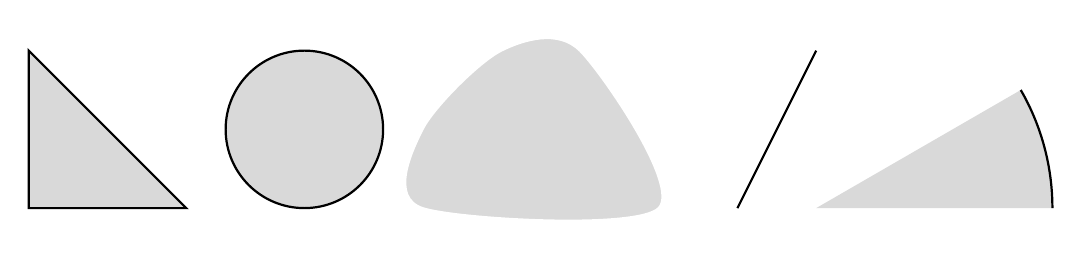
\begin{tikzpicture}[>=stealth', thick]

\draw [fill = gray!30] (0, 0)  --  ++ (0, 2)  -- ++ (2, -2)  --  cycle;
\draw [fill = gray!30] (3.5, 1) circle (1cm);

\begin{scope}[xshift = 5cm, yshift = 1cm]
    \draw [fill = gray!30, draw = white] plot [smooth cycle] coordinates {(0,0) (1,1) (2,1) (3,-1) (0,-1)};
    \draw (4, -1)  --  (5, 1);
\end{scope}

\begin{scope}[xshift = 10cm]
    \fill[fill = gray!30]
        (0,0)  --  (3cm,0cm) arc (0:30:3cm);
    \draw (3, 0) arc (0: 30: 3cm);
\end{scope}

% \node [scale = 1.3] at (6, -1) {Example of convex sets};
\end{tikzpicture}
\end{document}